\documentclass[10pt,letterpaper]{article}
\usepackage[margin=0.7in]{geometry}
\usepackage[T1]{fontenc}
\usepackage{graphicx}
\usepackage{booktabs}
\usepackage{enumitem}
\usepackage{titlesec}
\usepackage[font=small,labelfont=bf,skip=4pt]{caption}
\usepackage{xcolor}
\usepackage{tikz}
\usetikzlibrary{arrows.meta,positioning,fit,calc}
\usepackage[colorlinks=true,urlcolor=blue,linkcolor=black,citecolor=black]{hyperref}

% TODO: paste the Google Drive link to the demo video here.
\newcommand{\videolink}{\textcolor{red}{https://drive.google.com/file/d/1xmE9le1VtFV0ecj26mFJQgkK42axJxDS/view?usp=sharing}}

\titleformat{\section}{\normalfont\large\bfseries}{\thesection.}{0.4em}{}
\titlespacing*{\section}{0pt}{7pt}{3pt}
\setlist{nosep,leftmargin=1.3em}
\setlength{\parindent}{0pt}
\setlength{\parskip}{4pt}
\setlength{\textfloatsep}{8pt}
\setlength{\floatsep}{6pt}
\pagestyle{empty}

\begin{document}

\begin{center}
{\Large\bfseries Redactor: Select-Once Object Redaction for Video}\\[4pt]
CIS 5810 Final Project Proposal \textbullet{} Group 34 \textbullet{} Option 1\\[3pt]
\small
\begin{tabular}{ccc}
Kevin Song & AJ Boyle & Dhruv Gupta \\
\texttt{ksong37@engineering.upenn.edu} & \texttt{ajboyle@seas.upenn.edu} & \texttt{dhruvgup@engineering.upenn.edu}
\end{tabular}
\end{center}

\section{Goals and audience}

Anyone who posts footage of public places (journalists, researchers, people filming a street or an
event) eventually needs to hide a bystander, a face, or a license plate. Right now that means
keyframing a blur by hand, shot by shot. We want a tool where you say once what to hide and it stays
hidden for the rest of the clip. For now you do that by outlining the object on the first frame, but
we are building the pipeline so the request could also come from a detector or a text description.
We care most about leaks (the object should never be visible, even for a frame), and then about
keeping the mask tight so we don't blur the rest of the scene.

\section{Pipeline design}

We organized the pipeline around a single shared data type that we call the target prompt: a rough
region on some frame (a box or a coarse mask) plus an instance id. The stages before the prompt
decide what to hide. The stages after it work out where that thing is in each frame and hide it
(Figure~\ref{fig:pipeline}).

\begin{figure}[h]
\centering
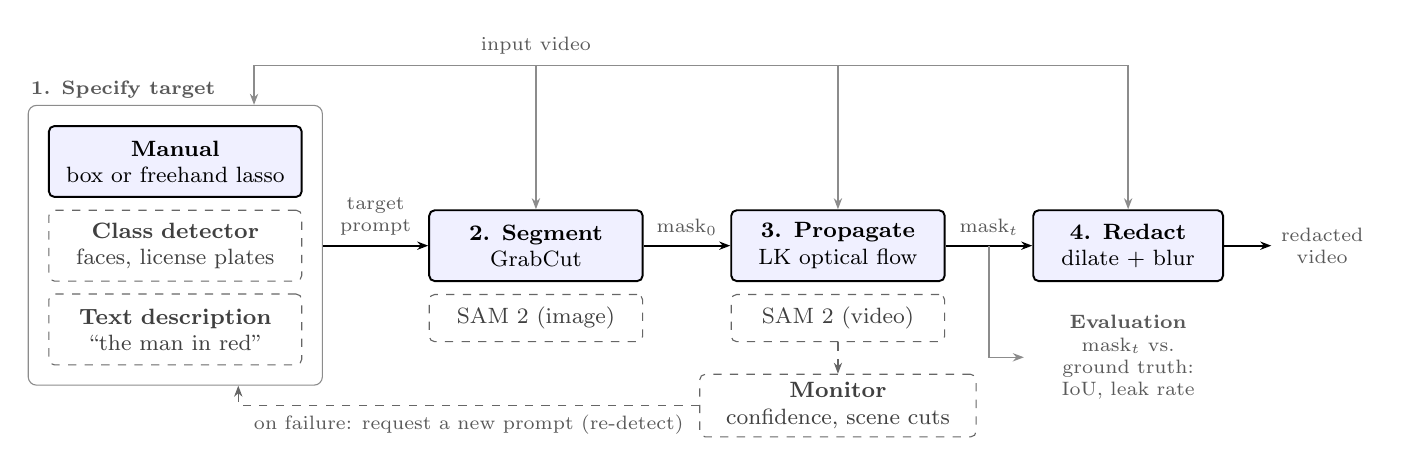
\begin{tikzpicture}[
  font=\footnotesize, >={Stealth[length=4pt]},
  box/.style={draw, rounded corners=2pt, align=center, inner sep=3pt, minimum height=9mm},
  built/.style={box, line width=0.7pt, fill=blue!6},
  plan/.style={box, dashed, draw=black!60, text=black!75},
  lab/.style={font=\scriptsize, text=black!65, align=center},
  flow/.style={->, line width=0.6pt},
  pflow/.style={->, dashed, draw=black!60},
]
% Stage 1: three interchangeable prompt sources
\node[built, text width=30mm] (manual) {\textbf{Manual}\\box or freehand lasso};
\node[plan, text width=30mm, below=1.5mm of manual] (detect) {\textbf{Class detector}\\faces, license plates};
\node[plan, text width=30mm, below=1.5mm of detect] (text) {\textbf{Text description}\\``the man in red''};
\node[draw=black!45, rounded corners=3pt, inner sep=2.5mm, fit=(manual)(detect)(text)] (specify) {};
\node[lab, anchor=south west, inner sep=1pt] at ($(specify.north west)+(0,0.4mm)$) {\textbf{1. Specify target}};

% Stages 2-4
\node[built, text width=25mm, right=16mm of detect] (segment) {\textbf{2. Segment}\\GrabCut};
\node[built, text width=25mm, right=11mm of segment] (propagate) {\textbf{3. Propagate}\\LK optical flow};
\node[built, text width=22mm, right=11mm of propagate] (redact) {\textbf{4. Redact}\\dilate + blur};
\node[plan, text width=25mm, minimum height=6mm, below=1.5mm of segment] (sam) {SAM 2 (image)};
\node[plan, text width=25mm, minimum height=6mm, below=1.5mm of propagate] (samv) {SAM 2 (video)};
\node[plan, text width=33mm, minimum height=6mm, below=4mm of samv] (monitor) {\textbf{Monitor}\\confidence, scene cuts};

% Video frames feeding each stage
\coordinate (bar) at ($(specify.north)+(0,5mm)$);
\node[lab, anchor=south] (video) at ($(segment.north |- bar)+(0,0.2mm)$) {input video};
\draw[black!45, line width=0.6pt] ($(specify.north |- bar)+(10mm,0)$) -- ($(redact.north |- bar)$);
\draw[flow, black!45] ($(specify.north |- bar)+(10mm,0)$) -- ($(specify.north)+(10mm,0)$);
\draw[flow, black!45] ($(segment.north |- bar)$) -- (segment.north);
\draw[flow, black!45] ($(propagate.north |- bar)$) -- (propagate.north);
\draw[flow, black!45] ($(redact.north |- bar)$) -- (redact.north);

% Main data flow
\draw[flow] (specify.east |- segment) -- node[lab, above] {target\\prompt} (segment);
\draw[flow] (segment) -- node[lab, above] {mask$_0$} (propagate);
\draw[flow] (propagate) -- node[lab, above] {mask$_t$} (redact);
\node[lab, right=6mm of redact] (out) {redacted\\video};
\draw[flow] (redact) -- (out);

% Planned feedback loop and evaluation tap
\draw[pflow] (samv) -- (monitor);
\draw[pflow] (monitor.west) -| node[lab, pos=0.25, below] {on failure: request a new prompt (re-detect)} ($(specify.south)+(8mm,0)$);
\node[lab, below=3mm of redact, text width=24mm] (eval) {\textbf{Evaluation}\\mask$_t$ vs.\ ground truth:\\IoU, leak rate};
\draw[->, black!45] ($(propagate.east)!0.5!(redact.west)$) |- (eval.west);
\end{tikzpicture}
\caption{Our pipeline. Every target source produces the same kind of prompt. Solid boxes are built,
dashed boxes are planned.}
\label{fig:pipeline}
\end{figure}

\begin{enumerate}
\item \textbf{Specify target:} Right now the user draws on the first frame and checks a preview of
the segmentation before anything runs. We want to add two more sources that plug into the same
interface. A class detector would propose every face or license plate with no user input. A text
description would go through an open-vocabulary detector such as Grounding DINO \cite{gdino}, which
returns boxes for a free-form phrase. These two behave differently from manual selection: they
return several instances at once and they can fire on any frame, so something that enters the clip
late still gets a prompt. The later stages will have to handle both.
\item \textbf{Segment:} GrabCut \cite{grabcut} turns the rough prompt into a pixel mask by fitting
color models to the foreground and background.
\item \textbf{Propagate:} We find Shi--Tomasi corners \cite{shitomasi} inside the current mask,
follow them into the next frame with pyramidal Lucas--Kanade flow \cite{lk}, and shift the mask by
their median displacement.
\item \textbf{Redact:} We dilate the mask with a $9{\times}9$ kernel as a safety margin and replace
that region with a $41{\times}41$ Gaussian blur.
\end{enumerate}

\textbf{Why this design:} We wanted to be able to swap out one stage and measure it on its own,
which works because the benchmark reads the mask between stages 3 and 4. We started with classical
methods because they need only a CPU and OpenCV, and when they fail you can see why. That gives us
something concrete to compare SAM 2 against in stages 2 and 3. The monitor is the piece we are
missing today: when confidence drops or the scene cuts, it should ask stage 1 for a new prompt.

\section{Baseline results}

\textbf{Baseline:} The user drags a bounding box, GrabCut is initialized from that rectangle, and
propagation is the translation-only tracker described above.

\textbf{Evaluation:} We don't have annotated real footage yet, so we wrote a synthetic benchmark
(\texttt{scripts/evaluate.py}). It renders a textured, person-shaped object over a cluttered
background, which gives us exact ground-truth masks. There are four 90-frame clips, each testing one
thing: plain translation, scale change (the object shrinks to 45\% as it walks away), occlusion (it
passes completely behind a pillar), and a scene cut at frame 45. We simulate the user's prompt from
the ground truth with 5, 9 and 13 pixels of slack and average the three runs. We report mask IoU
against the visible object and a leak rate, which is the fraction of visible object pixels still
unblurred after the safety dilation. For a privacy tool the leak rate is the number we care about
most.

\begin{table}[h]
\centering\small
\setlength{\tabcolsep}{4.5pt}
\begin{tabular}{lccccccccc}
\toprule
 & Frame 0 & \multicolumn{2}{c}{Translation} & \multicolumn{2}{c}{Scale} &
 \multicolumn{2}{c}{Occlusion} & \multicolumn{2}{c}{Scene cut} \\
\cmidrule(lr){3-4}\cmidrule(lr){5-6}\cmidrule(lr){7-8}\cmidrule(lr){9-10}
Method & IoU & IoU & Leak & IoU & Leak & IoU & Leak & IoU & Leak \\
\midrule
Baseline: box + GrabCut + LK translation   & 0.87 & 0.85 & 0\% & 0.41 & 22\% & 0.37 & 49\% & 0.43 & 50\% \\
Iteration 1: lasso + seeded GrabCut        & 0.84 & 0.84 & 0\% & 0.42 & 18\% & 0.36 & 49\% & 0.42 & 50\% \\
Iteration 1 + occlusion gate (prototype)   & 0.84 & 0.84 & 0\% & 0.42 & 17\% & 0.36 & 49\% & 0.42 & 50\% \\
\bottomrule
\end{tabular}
\caption{Mean mask IoU (higher is better) and mean leak rate (lower is better) over each
90-frame synthetic clip.}
\label{tab:results}
\end{table}

The baseline does fine when the object only translates (IoU 0.85, no leak) and breaks in the other
three clips (Figure~\ref{fig:curves}). When the object shrinks, the mask stays its original size and
slides off, hitting IoU 0 by frame 80. In the occlusion clip the mask gets stuck at the edge of the
pillar and never catches up, so IoU is 0 for every frame after the object comes back out. After the
scene cut the mask just stays where it was, and the object is fully exposed for the rest of the clip.

\begin{figure}[h]
\centering
\includegraphics[width=\linewidth]{figures/iou_curves.pdf}
\caption{Mask IoU per frame on the synthetic clips. The gap under occlusion is where the object is
fully hidden.}
\label{fig:curves}
\end{figure}

\section{Iteration 1 results}

\textbf{Change:} A box is a poor fit for a pedestrian in a crowd, because a rectangle around one
person also picks up parts of the people next to them. So we replaced the box with a freehand lasso
and seeded GrabCut from it. Pixels deep inside the outline (more than 35\% of the maximum distance
from its edge) are marked definite foreground, the rest of the outline is probable foreground, a
thin band just outside is probable background, and everything else is definite background.
Propagation and redaction did not change.

\textbf{Synthetic result:} On the benchmark the lasso did not help (Table~\ref{tab:results}).
First-frame IoU is 0.84 versus 0.87 for the box, and the tracking numbers are within 0.01 IoU of the
baseline in every clip. We think this is because the synthetic object stands alone, so either prompt
gives GrabCut enough to work with. The benchmark can't show what the lasso is for, and we will need
crowded real frames with annotated masks to measure that. It also tells us that segmentation is not
what is holding us back. Every failure in Table~\ref{tab:results} comes from propagation.

\textbf{Real footage:} Figure~\ref{fig:real} shows Iteration 1 on a 5-second clip of a crowded
crosswalk ($2320{\times}1080$, 150 frames). The selection on frame 0 looks right. By frame 75 the
blur is lagging behind the subject and covering part of the person next to her. By frame 148 she has
walked away and gotten smaller, the mask has not, and it is now blurring bystanders in the
foreground while she is fully visible. This is the same scale failure we saw on the benchmark, plus
drift onto nearby people. Video: \videolink.

\begin{figure}[h]
\centering
\includegraphics[width=0.88\linewidth]{figures/crosswalk.jpg}
\caption{Iteration 1 on real footage (frames 0, 75, 148). Top: input. Bottom: output. Subject: the
woman in the white skirt.}
\label{fig:real}
\end{figure}

\textbf{Occlusion gate (prototyped, then removed):} We also tried to catch bad motion estimates with
a forward-backward check \cite{fb}: track the points forward, track them back, and keep the ones
that land within 1.5 pixels of where they started. If fewer than three survive, or the jump is over
20 pixels, we freeze the mask. It made no difference (Table~\ref{tab:results}). On the occlusion
clip the gate never fired, because the points that are left as the object disappears still pass the
check, and the mask gets stuck at the pillar just like before. On the scene-cut clip it fired on
every frame after the cut, but a frozen mask does not find the object again, so we took it out.
Noticing a failure does not help unless we can also re-detect the object.

\newpage
\section{Plan for improvements}

Each iteration changes one stage, and we score it on the same benchmark. Items 2--4 go after the
scale, occlusion and scene-cut clips in that order.

\begin{enumerate}
\item \textbf{Evaluation on real video:} Add sequences from DAVIS 2017 \cite{davis}, which comes
with per-frame object masks and has sequences with occlusion and scale change. We will also annotate
frames from our own crosswalk footage.
\item \textbf{Scale-aware propagation:} Fit a similarity transform to the tracked points with RANSAC
instead of using the median translation, and re-run GrabCut on the propagated mask every few frames
to keep it from drifting.
\item \textbf{Occlusion recovery:} Keep an appearance model of the object from frame 0 (a color
histogram first, learned features later). When confidence drops, hold the mask on its predicted path
and search for the object.
\item \textbf{Scene cuts:} Detect cuts from the frame-to-frame histogram difference, then trigger
the same re-detection, or stop redacting if the object is gone.
\item \textbf{SAM 2:} Replace stages 2 and 3 with SAM 2 \cite{sam2}, which propagates a prompted
mask through a video using a memory of past frames and is built to handle occlusion and
reappearance. We will compare it with our classical pipeline on accuracy and speed.
\item \textbf{New target sources:} Add the class detector (faces, license plates) and then the
text-description source \cite{gdino} to stage 1. This also means extending propagation to several
instances and to prompts that arrive mid-clip.
\end{enumerate}

\section{Timeline, milestones, and member duties}

\begin{center}
\small
\begin{tabular}{lll}
\toprule
Dates & Milestone & Lead \\
\midrule
10/12--10/25 & Real-video benchmark (DAVIS + annotated crosswalk frames); first TA meeting & Dhruv \\
10/19--11/1  & Scale-aware propagation with periodic re-segmentation & Kevin \\
10/26--11/8  & SAM 2 integrated as an alternative segment/propagate backend & AJ \\
11/2--11/15  & Occlusion recovery and scene-cut handling & Kevin \\
11/20        & Midterm report: three iterations compared on the benchmark & All \\
11/21--12/3  & Detector and text-description target sources; UI polish & AJ, Dhruv \\
12/6         & Final Project Day demo & All \\
12/10        & Final report, demo video, code & All \\
\bottomrule
\end{tabular}
\end{center}

\textbf{Duties:} Kevin is taking propagation (tracking, occlusion, cuts). AJ is taking target
selection and segmentation, including SAM~2. Dhruv is taking the evaluation data and metrics, plus
the detector and text sources.

\textbf{TA request:} None.

\textbf{Generative AI use:} Claude Code (Anthropic) has been used for helping develop evaluation scripts and graphs, and for drafting ideas of where to take this project for this proposal

{\footnotesize
\begin{thebibliography}{9}
\setlength{\itemsep}{0pt}
\bibitem{grabcut} C. Rother, V. Kolmogorov, A. Blake. GrabCut: Interactive foreground extraction
using iterated graph cuts. \emph{SIGGRAPH}, 2004.
\bibitem{shitomasi} J. Shi, C. Tomasi. Good features to track. \emph{CVPR}, 1994.
\bibitem{lk} B. Lucas, T. Kanade. An iterative image registration technique with an application to
stereo vision. \emph{IJCAI}, 1981.
\bibitem{fb} Z. Kalal, K. Mikolajczyk, J. Matas. Forward-backward error: Automatic detection of
tracking failures. \emph{ICPR}, 2010.
\bibitem{davis} J. Pont-Tuset et al. The 2017 DAVIS challenge on video object segmentation.
\emph{arXiv:1704.00675}, 2017.
\bibitem{sam2} N. Ravi et al. SAM 2: Segment anything in images and videos.
\emph{arXiv:2408.00714}, 2024.
\bibitem{gdino} S. Liu et al. Grounding DINO: Marrying DINO with grounded pre-training for open-set
object detection. \emph{arXiv:2303.05499}, 2023.
\end{thebibliography}
}

\end{document}
